%!Mode:: "TeX:UTF-8"
%!TEX program  = xelatex
\documentclass[bwprint]{cumcmthesis}
%\documentclass[withoutpreface,bwprint]{cumcmthesis} %去掉封面与编号页

\usepackage{tikz,mathpazo}
\usetikzlibrary{shapes.geometric, arrows}

\title{平行束CT系统参数标定及成像}
\tihao{A}
\baominghao{报名号}
\schoolname{中国人民解放军陆军军医大学}
\membera{唐凯}
\memberb{王艺超}
\memberc{李翔}
\supervisor{宋丽娟}
\yearinput{2017}
\monthinput{9}
\dayinput{11}
\begin{document}
 \maketitle
 \begin{abstract}
 CT作为一种重要的无损检测技术已广泛应用于国防,医学影响和化工等领域。本文将对平行束CT系统参数标定及成像问题进行探索和研究。具体研究内容如下:
问题一,通过分析探测器接收到的信息以及托盘内两个标定模版的位置信息,可以得到4个探测器单元之间距离的近似值,我们把这4个近似值取平均值(0.2765mm)作为探测器单元之间距离的最终值。然后,通过分析射线平行于X轴和Y轴入射时探测器单元接收到的信息以及探测器正对于托盘中心旋转时,和探测器正对于旋转中心旋转时的位置关系,确定了旋转中心相对于托盘中心的偏移量,进而求得了旋转中心的坐标 mm。最后,我们在探测器接受到的数据中定位到了射线平行于X轴入射时(0°),以及射线平行于Y轴入射时(90°)的两列数据,而这两列列数的差值为90,进而推算出CT每旋转一次的方向恰为1°,继而得到其余180个方向的角度范围为-60度到120度。
问题二,我们依据CT扫描原理建立了平行束二维CT系统成像标定模型,该模型将CT扫描后得到的待标定图像f(x,y)进行旋转、平移、还有大小调整转化为实际扫描时介质的图像G(x,y)。然后通过将正方形托盘实际边长与像素点的换算,以及托盘中心和旋转中心的相对位置,进而在以旋转中心为原点,平行和垂直于于托盘左边X、Y轴的平面直角坐标系中将托盘和介质都绘制出来,继而可通过取点计算得到该介质上任何一点的坐标。最后,我们将标定图像内Radon逆转换的362×362数据缩放为256×256的数据(即射线吸收率数据)并生成为problem2.xls,将附件4中10个点根据坐标一一对应与该数据表进而求得这十个点的射线吸收率。其中第2、4、5、6、7处位置的吸收率为0.4878、1.1838、1.0331、1.4820、1.2729,其余吸收率为0.0000。
问题三,我们使用了Radon逆转换将附件数据还原为待标定图片。然后利用问题二所建立的模型将托盘和还原后的图片共同绘制在如问题二所述的平面直角坐标系中。最后,同问题二将缩放后的256×256的数据(即射线吸收率数据)生成为problem3.xls,将附件4中10个点根据坐标一一对应与该数据表进而求得这十个点的射线吸收率。其中第2、3、5、6、7、9处位置的吸收率为1.8413、5.2027、0.9190、2.2433、4.8737和5.6109,其余吸收率为0.0000。
问题四,基于问题一的计算过程,我们分别将探测器单元距离,旋转中心较托盘中心的坐标偏移量以及探测器每旋转一个方向时的角度可能的取值取出,代入到问题二中未知介质的CT扫描情形下对其进行标定,通过计算并比较各取值条件下圆盘中心点(0,0)的吸收率,并计算吸收率方差,得到我们模型标定的稳定性较高的结论。由于各个参数取值较多,故标定精度相对较差。为了进一步提高标定时的精度和稳定度,我们设计了一个较为锐利的等腰直角三角形图案,再次利用上述方法求得圆盘中心点(0,0)的吸收率,因其方差接近于0故稳定性较好。参数取值较之前问题有明显减少,故精度提高。
综上所述,本文通过建立平行束二维CT系统图像标定模型,较好的实现了CT图像的标定和吸收率的求解,通过设计新的标定模板使得稳定性和精度均较之前有明显提高。


\keywords{ CT\quad  平行束\quad 吸收率\quad  发射-接收系统}
\end{abstract}

\section{问题重述}
CT(Computed Tomography)可以在不破坏样品的情况下,利用样品对射线能量的吸收特性对生物组织和工程材料的样品进行断层成像,由此获取样品内部的结构信息。一种典型的二维CT系统如图1所示,平行入射的X射线垂直于探测器平面,每个探测器单元看成一个接收点,且等距排列。X射线的发射器和探测器相对位置固定不变,整个发射-接收系统绕某固定的旋转中心逆时针旋转180次。对每一个X射线方向,在具有512个等距单元的探测器上测量经位置固定不动的二维待检测介质吸收衰减后的射线能量,并经过增益等处理后得到180组接收信息。
CT系统安装时往往存在误差,从而影响成像质量,因此需要对安装好的CT系统进行参数标定,即借助于已知结构的样品(称为模板)标定CT系统的参数,并据此对未知结构的样品进行成像。
请建立相应的数学模型和算法,解决以下问题:
\begin{description}
\item (1)在正方形托盘上放置两个均匀固体介质组成的标定模板,模板的几何信息如图2所示,相应的数据文件见附件1,其中每一点的数值反映了该点的吸收强度,这里称为"吸收率"。对应于该模板的接收信息见附件2。请根据这一模板及其接收信息,确定CT系统旋转中心在正方形托盘中的位置、探测器单元之间的距离以及该CT系统使用的X射线的180个方向。
\item (2) 附件3是利用上述CT系统得到的某未知介质的接收信息。利用(1)中得到的标定参数,确定该未知介质在正方形托盘中的位置、几何形状和吸收率等信息。另外,请具体给出图3所给的10个位置处的吸收率,相应的数据文件见附件4。
\item (3) 附件5是利用上述CT系统得到的另一个未知介质的接收信息。利用(1)中得到的标定参数,给出该未知介质的相关信息。另外,请具体给出图3所给的10个位置处的吸收率。
\item (4) 分析(1)中参数标定的精度和稳定性。在此基础上自行设计新模板、建立对应的标定模型,以改进标定精度和稳定性,并说明理由。
\end{description}


\section{模型假设}
\begin{enumerate}
	\item 二维CT系统每次转动时转动的角度相同。
	\item 二维CT系统的发射器和探测器之间的距离大于正方形托盘对角线。
	\item 二维CT系统工作时不受其产生的电磁场等其他因素的干扰。
\end{enumerate}



\section{符号说明}
\begin{tabular}{cc}
	\hline
	\makebox[0.3\textwidth][c]{符号}	&  \makebox[0.6\textwidth][c]{定义} \\ \hline
    $\textit{a}_{i} $ & 去 0 处理后的信息\\ \hline
	$\textit{n}_{i} $ & $a_{i}$对应信息的长度 \\ \hline
	\textit{d} & 相邻两单元之间的距离 \\ \hline
	$\Delta$$\textit{x}$、$\Delta$$\textit{y}$ & X轴、Y轴方向的偏移量 \\ \hline
	$\Delta$$\overline{\theta}$ & 每转动一次转过的角度 \\ \hline
	$\varphi$ & 标定时的旋转角度 \\ \hline
	$\mu$ & 吸收率 \\ \hline
	
\end{tabular}

\section{问题分析}
CT(computed tomography)作为一种重要的无损检测技术已广泛应用于国防,医学 影响和化工等领域。本文拟对平行束 CT 系统参数标定及成像问题进行建模和研究。
\subsection{问题一}
问题一要求我们根据标定模板在 CT 系统成像时的相关信息,确定 CT 系统旋转中 心在正方形托盘中的位置、探测器单元之间的距离以及该 CT 系统使用的 X 射线的 180 个方向。 我们首先确立了以椭圆中心为原点,短轴所在延长线为 X 轴(正方向为右),长轴 所在延长线为 Y 轴(正方向为上)的直角坐标系。通过分析探测器接收到的信息以及托 盘内两个标定模版的位置信息,我们计算得到了每个探测器单元之间的距离。然后,通 过分析射线平行于 X 轴和 Y 轴入射时探测器单元接收到的信息以及探测器正对于托盘 中心旋转时,和探测器正对于旋转中心旋转时的位置关系,确定了旋转中心相对于托盘 中心的偏移量,进而求得了旋转中心的坐标。最后,我们在探测器接收到的数据中确定 了平行于 X 轴和 Y 轴时探测器所在的角度,进而根据假设一推算出了探测器旋转时 180 个方向的角度。

\subsection{问题二}
问题二要求我们利用上述 CT 系统得到的某未知介质的接收信息,以及问题一中得 到的标定参数,确定该未知介质在正方形托盘中的位置、几何形状和吸收率等信息。还 要求我们具体给出 10 个图中位置的吸收率。 首先,我们根据 CT 成像原理以及问题一求得的标定参数建立了平行束二维 CT 系 统图像标定模型。该模型可将 CT 扫描后得到的待标定图像进行旋转,平移,还有大小 调整转化为实际扫描时介质的形态。然后通过将正方形托盘实际边长与像素点的换算, 以及托盘中心和旋转中心的相对位置,进而在以旋转中心为原点,平行和垂直于于托盘 左边 X、Y 轴的平面直角坐标系中将托盘和介质都绘制出来,继而可通过取点计算得到 该介质上任何一点的坐标。最后,我们将待标定图像进行调整时 Radon 逆函数所求得的 数值缩放为 256×256 的数据(即射线吸收率数据),将附件 4 中 10 个点根据坐标一一 对应与该数据表进而求得这十个点的射线吸收率。
\subsection{问题三}
问题三要求我们利用另一个未知介质的 CT 接收信息以及之前所求得的标定参数, 给出该未知介质的相关信息。另外,请具体给出图 3 所给的 10 个位置处的吸收率。 首先,我们利用问题二中所建立的模型将图片还原为 CT 扫描时的实际形态。然后 利用正方形托盘中心与旋转中心的相对位置,以及实际边长与像素点的换算关系,将托 盘和还原后的图片共同绘制在如问题二所述的平面直角坐标系中。最后,同问题二,将 Radon 逆函数求得的数据缩放,进而可求得未知介质以及附件 4 中 10 个位置的吸收率。

\subsection{问题四}
问题四要求我们分析问题一中参数标定的精度和稳定性。在此基础上自行设计新模 板、建立对应的标定模型,以改进标定精度和稳定性,并说明理由。 首先,基于问题一的计算过程,我们对于探测器单元距离,旋转中心较托盘中心的 坐标偏移量以及探测器每旋转一个方向时的角度进行可能的取值分析。将各个变量的可 能取值代入到问题二中未知介质的 CT 扫描情形下对其进行标定,通过计算并比较各取 值条件下圆盘中心的吸收率进而探究问题一中参数标定的稳定性程度。对于参数标定的 精度,我们主要通过各个参数可能的取值范围来讨论。 然后,为了进一步提高标定时的提高精度和稳定度,我们设计了一个较为锐利的等 腰直角三角形图案(边缘有缺损),利用问题一中的方法和问题二中所建立的二维 CT系统图像标定模型再次计算相关参数。通过分析其求解过程中各参数可能的取值,以及 各取值情况下圆盘中心的吸收率观察参数标定的稳定性以及精度。
\subsection{思路总结}
综上所述,对于平行束 CT 系统参数标定及成像问题问题可以通过下图所示流程图进行 求解
%绘图

%\begin{tikzpicture}
%    [every node/.style={fill=blue!30,draw=white!70,rounded corners},
%     edge from parent/.style={thick,draw}]
%%        \node (a){a}
%        \node [below of=a]{root}
%            child {node {a1}}
%            child {node {a2}
%                child {node {b1}}
%                child {node {b2}}}
%            child {node {a3}};
% \end{tikzpicture}

%% 流程图定义基本形状
%\tikzstyle{startstop} = [rectangle, rounded corners, minimum width=3cm, minimum height=1cm,text centered, draw=black, fill=red!30]
%\tikzstyle{io} = [trapezium, trapezium left angle=70, trapezium right angle=110, minimum width=3cm, minimum height=1cm, text centered, draw=black, fill=blue!30]
%\tikzstyle{process} = [rectangle, minimum width=3cm, minimum height=1cm, text centered, draw=black, fill=orange!30]
%\tikzstyle{decision} = [diamond, minimum width=3cm, minimum height=1cm, text centered, draw=black, fill=green!30]
%\tikzstyle{arrow} = [thick,-&gt;,&gt;=stealth]
% 
%\begin{center}
%
%\begin{tikzpicture}[node distance=2cm]
% %定义流程图具体形状
%\node (start) [startstop] {Start};
%\node (in1) [io, below of=start] {Input};
%\node (pro1) [process, below of=in1] {Process 1};
%\node (dec1) [decision, below of=pro1, yshift=-0.5cm] {Decision 1};
%\node (pro2a) [process, below of=dec1, yshift=-0.5cm] {Process 2a};
%\node (pro2b) [process, right of=dec1, xshift=2cm] {Process 2b};
%\node (out1) [io, below of=pro2a] {Output};
%\node (stop) [startstop, below of=out1] {Stop};
% 
% %连接具体形状
%\draw [->,ultra thick](start) -- (in1);
%\draw [->,ultra thick](in1) -- (pro1);
%\draw [->,ultra thick](pro1) -- (dec1);
%\draw [->,ultra thick](dec1) -- (pro2a);
%\draw [->,ultra thick](dec1) -- (pro2b);
%\draw [->,ultra thick](dec1) -- node[anchor=east] {yes} (pro2a);
%\draw [->,ultra thick](dec1) -- node[anchor=south] {no} (pro2b);
%\draw [->,ultra thick](pro2b) |- (pro1);
%%\draw [->](pro2a) -- (out1);
%%\draw [->](out1) -- (stop);
%\end{tikzpicture}
%\end{center}
%%%%%%%%%%%%%%%%%%%
\subsection{模型的建立与求解}
\subsection{问题一:CT系统参数的标定}
\subsubsection{平面直角坐标系的建立}
以正方形托盘中心为原点,分别以椭圆短轴为 X 轴方向,长轴方向为 Y 轴方向建立如所示的坐标系。设椭圆和圆中心的坐标分别为,其坐标经计算分别为。
%%%%%图1
\begin{figure}[htbp]
\centering
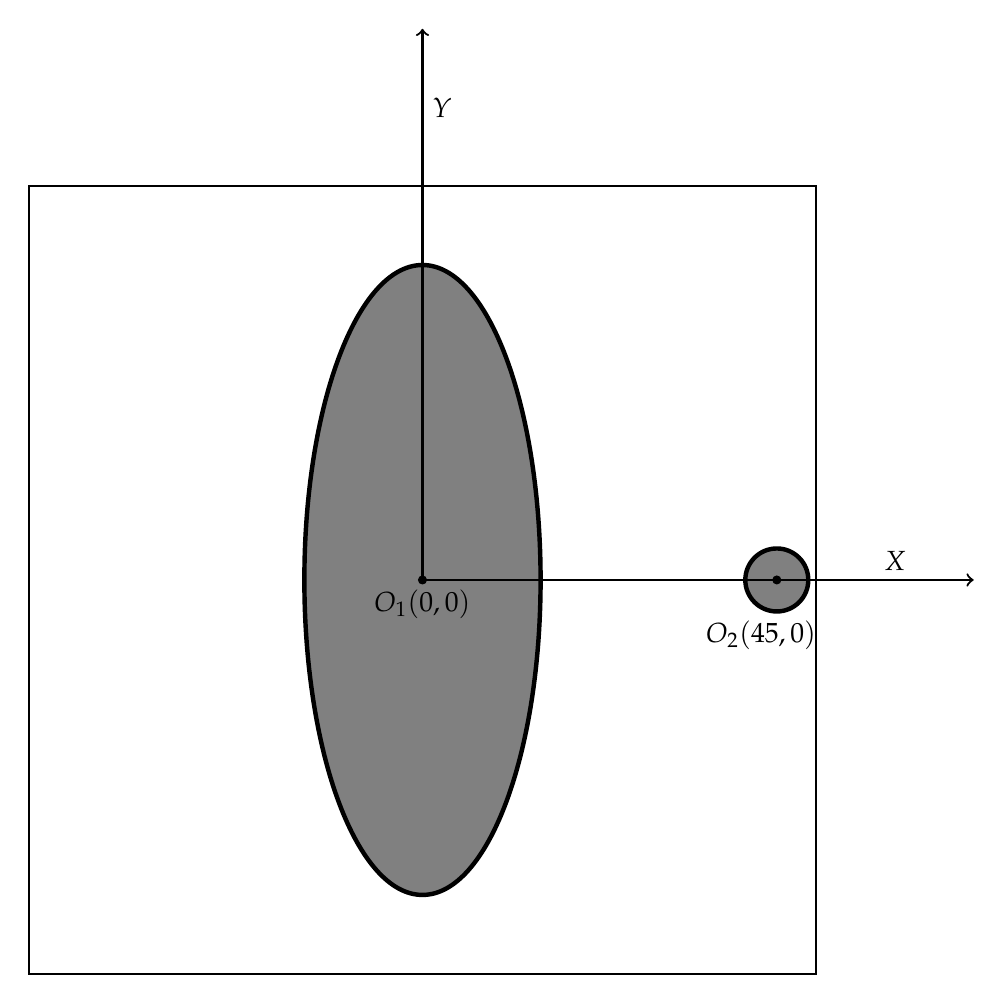
\begin{tikzpicture} 
	\draw [thick] (-50mm,-50mm) rectangle (50mm,50mm);
	\draw [fill=gray, ultra thick] (0mm,0mm) ellipse (15mm and 40mm);
	\draw [fill=gray, ultra thick] (45mm,0mm) circle [radius=4mm];
	\draw [<->, thick] (0mm,70mm)--(0,0)--(70mm,0);
	\draw [fill](0,0) circle [radius=0.5mm];
	\node [below] at (0,0) {$O_1 (0,0)$};
	\draw [fill](45mm,0) circle [radius=0.5mm];
	\node [below] at (43mm,-4mm) {$O_2 (45,0)$};
	\node [above] at (60mm,0) {$\textit{X}$};
	\node [right] at (0mm,60mm) {$\textit{Y}$};
\end{tikzpicture}
\caption{参数标定平面直角坐标系}
\end{figure}
%%%%%%%
\subsection{二维 CT 照射分析}
为便于分析理解,我们取射线方向平行于 X 轴方向与射线方向平行于 Y 轴方向时的 情况进行分析。
当射线方向平行于 X 轴方向照射时(如图\ref{附件2中第61个方向示意}),射线此时穿过的椭圆截面是 其环绕一圈中最大的,即此时位于图中 l 4 范围内的探测器均可以探测到标定物的吸收信息。在附件2的数据中(如图 3 所示),横向的 180 列代表的是 180 个方向,纵向的 512 行代表的是探测器单元。因此,若我们认为每个单元格是一个像素的情况下,射线平行 X 轴照射时对应于图 3 中的 n 4 (其所对应的数据列数为 61 列),即接此时是收到信息的 探测器数量最多的情形。
同理,当射线方向平行于 Y 轴方向照射时(如图 2-2 所示),l 1 和 l 2 范围内的探测 器将可以分布探测到椭圆和圆两者的信息(分别对应于图 3 中的 n 1 , n 2 )。此外,椭圆 和圆的间距此时在探测器上的投影也是 CT 成像过程中最大的时候(分别对应于图 3 中 的 n 3 ,其所对应的数据列数为 151 列)。

不仅如此,在两种状态下,过椭圆中心的射线穿过的物体距离最长(平行于 Y 轴的 射线过椭圆终点被探测器接受到的数据位于图三中的 n 5 位置)。

%%%%%%%%%%%%%%%并排放

\begin{figure}[htbp]
\centering
\begin{minipage}{2pt}
\centering
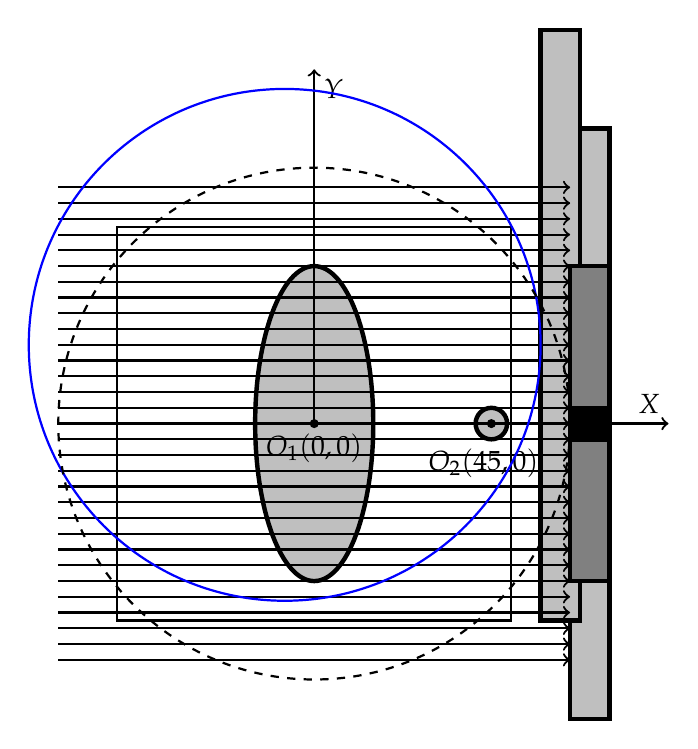
\begin{tikzpicture}[scale=0.5]%射线方向平行于X方向

%\draw[help lines] (-100mm,-100mm) grid (100mm,100mm);

	\draw [thick] (-50mm,-50mm) rectangle (50mm,50mm);%基本矩形
	\draw [fill=lightgray, ultra thick] (65mm,-75mm) rectangle(75mm,75mm);%接收板
	\draw [fill=lightgray, ultra thick] (57.5mm,-50mm) rectangle(67.5mm,100mm);%运动接收板
	
	\draw [fill=lightgray, ultra thick] (0mm,0mm) ellipse (15mm and 40mm);%椭圆
	\draw [fill=lightgray, ultra thick] (45mm,0mm) circle [radius=4mm];%小圆
	\draw [<->, thick] (0mm,90mm)--(0,0)--(90mm,0);
	\node [below] at (0,0) {$O_1 (0,0)$};
	\draw [fill](0,0) circle [radius=1mm];
	\draw [fill](45mm,0) circle [radius=1mm];
	\node [below] at (43mm,-4mm) {$O_2 (45,0)$};
	\node [above] at (85mm,0) {$\textit{X}$};
	\node [right] at (0mm,85mm) {$\textit{Y}$};
%	\draw (0,-100mm)--(0,100mm);%辅助线
%	\draw (-100mm,0)--(100mm,0);%辅助线
	\foreach \i in {-15,-14,...,15}
	\draw [thick,->] (-65mm, \i*4mm)--(65mm, \i*4mm);%画射线
	\draw [fill=gray, ultra thick] (65mm,-40mm) rectangle(75mm,40mm);%椭圆投影
	\draw [fill=black, ultra thick] (65mm,-4mm) rectangle(75mm,4mm);%圆投影
	\draw [blue,thick]  (-7.5mm,20mm)circle[radius=65mm];%运动轨迹
	\draw [dashed,thick] (0,0) circle[radius=65mm];%运动轨迹虚线
	\end{tikzpicture}
	\caption{\small{附件2中第61个方向示意}}
	\label{附件2中第61个方向示意}
	

\end{minipage}
\hspace{80mm}%
\begin{minipage}{2pt}


	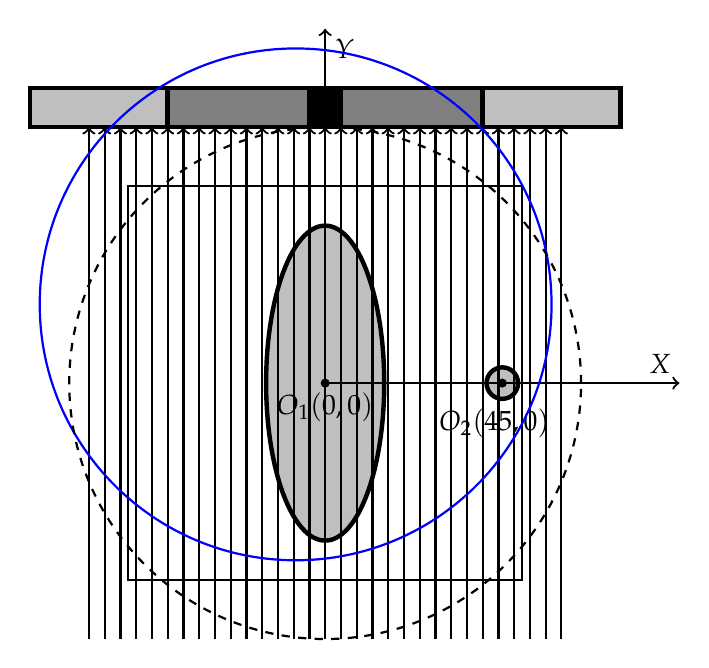
\begin{tikzpicture}[scale=0.5] %%%%%61个方向Y方向

%\draw[help lines] (-100mm,-100mm) grid (100mm,100mm);

	\draw [thick] (-50mm,-50mm) rectangle (50mm,50mm);%基本矩形
	\draw [fill=lightgray, ultra thick] (-75mm,65mm) rectangle(75mm,75mm);%接收板
	
	\draw [fill=lightgray, ultra thick] (0mm,0mm) ellipse (15mm and 40mm);%椭圆
	\draw [fill=lightgray, ultra thick] (45mm,0mm) circle [radius=4mm];%小圆
	\draw [<->, thick] (0mm,90mm)--(0,0)--(90mm,0);%坐标轴
	\node [below] at (0,0) {$O_1 (0,0)$};
	\draw [fill](0,0) circle [radius=1mm];%O1点
	\draw [fill](45mm,0) circle [radius=1mm];%O2点
	\node [below] at (43mm,-4mm) {$O_2 (45,0)$};
	\node [above] at (85mm,0) {$\textit{X}$};
	\node [right] at (0mm,85mm) {$\textit{Y}$};
%	\draw (0,-100mm)--(0,100mm);%辅助线
%	\draw (-100mm,0)--(100mm,0);%辅助线
	\foreach \i in {-15,-14,...,15}
	\draw [thick,->] (\i*4mm,-65mm)--(\i*4mm, 65mm);%画射线
	\draw [fill=gray, ultra thick] (-40mm,65mm) rectangle(40mm,75mm);%椭圆投影
	\draw [fill=black, ultra thick] (-4mm,65mm) rectangle(4mm,75mm);%圆投影
	\draw [blue,thick]  (-7.5mm,20mm)circle[radius=65mm];%运动轨迹
	\draw [dashed,thick] (0,0) circle[radius=65mm];%运动轨迹虚线
	
	\end{tikzpicture}
	\caption{\small{附件 2 中第 151 个方向示意}}
\end{minipage}
\end{figure}

\begin{tikzpicture} 
\draw [<->, thick] (0mm,90mm)--(0,0)--(90mm,0);%坐标轴
\draw (0,3) parabola bend (3,5) (7.5,4); 
\draw (7.5,4) parabola bend (9,4.5) (9,4.5); %上界

\draw (0,1) parabola bend (3,1) (7.5,2); 
\draw (7.5,2) parabola bend (9,1) (9,1);
\draw (0,0.5) parabola bend (7.5,6) (9,5); 
\draw (0,0) parabola bend (7.5,5.5) (9,4.5); 
\draw (9,4.5)--(9,5);

\end{tikzpicture}

\subsection{探测器单元之间的距离求解}
经过上述分析,我们可通过求可探测到信息的探测器范围的总长度除以探测器单元 的数量,进而得到探测器之间的距离,如下式所示:
\[\textit{d}_i=(\frac{\textit{t}_i}{\textit{n}_i}), i=1,2,3,4\]



\subsection{公式1}


\[
\begin{pmatrix}{*{20}c}
{a_{11} } & {a_{12} } & {a_{13} }  \\
{a_{21} } & {a_{22} } & {a_{23} }  \\
{a_{31} } & {a_{32} } & {a_{33} }  \\
\end{pmatrix}
= \frac{{Opposite}}{{Hypotenuse}}\cos ^{ - 1} \theta \arcsin \theta
\]

\subsection{公式2}

\[
p_{j}=\begin{cases} 0,&\text{if $j$ is odd}\\
r!\,(-1)^{j/2},&\text{if $j$ is even}
\end{cases}
\]

\subsection{公式3}

\[
\arcsin \theta  =
\mathop{{\int\!\!\!\!\!\int\!\!\!\!\!\int}\mkern-31.2mu
	\bigodot}\limits_\varphi
{\mathop {\lim }\limits_{x \to \infty } \frac{{n!}}{{r!\left( {n - r}
			\right)!}}} \eqno (1)
\]

\section{表格}

\begin{tabular}{cc}
	\hline
	\makebox[0.4\textwidth][c]{C1}	&  \makebox[0.5\textwidth][c]{C2} \\ \hline
	A	    & 中文测试\\ \hline
	B	    & 中文测试 \\ \hline
	C	    & 中文测试 \\ \hline
\end{tabular}

\section{图片}

\subsection{eps}

\begin{figure}[h]
	\centering
	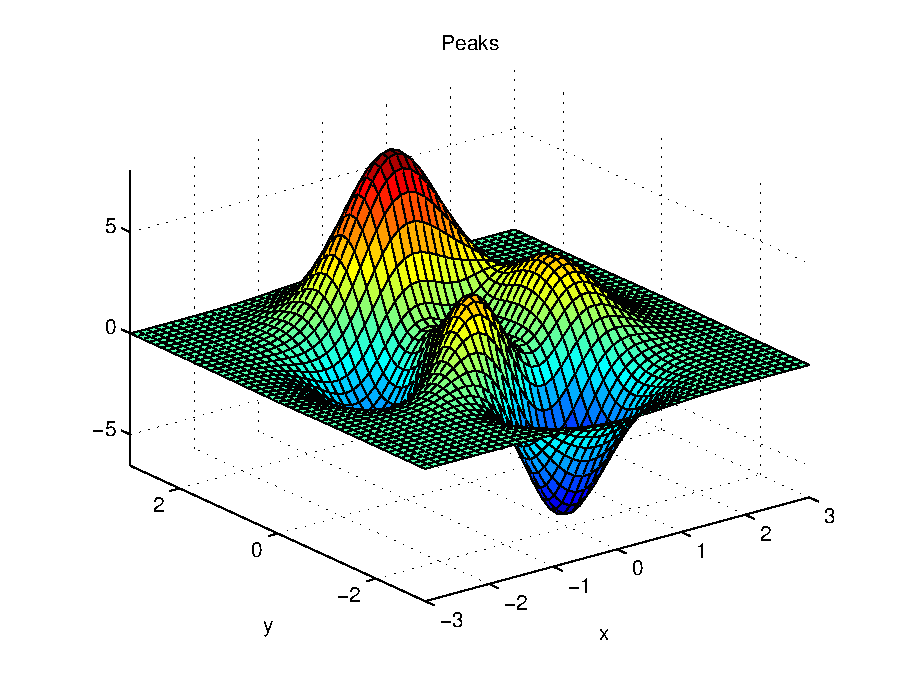
\includegraphics[width=\textwidth]{eps.eps}
	\caption{eps}
\end{figure}
\clearpage
\subsection{pdf}

\begin{figure}[h]
	\centering
	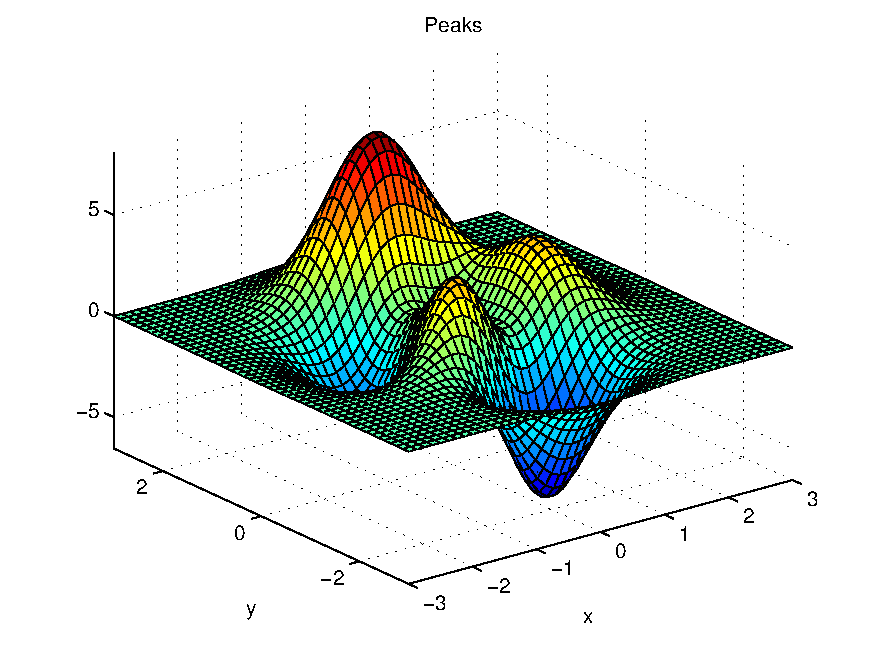
\includegraphics[width=\textwidth]{pdf.pdf}
	\caption{pdf}
\end{figure}
\clearpage
\subsection{jpg}

\begin{figure}[h]
	\small
	\centering
	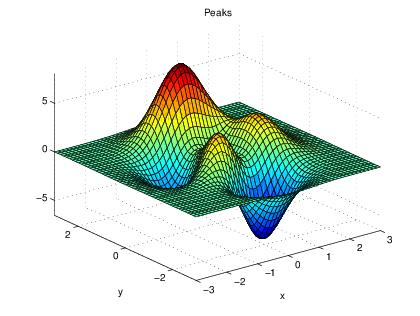
\includegraphics[width=12cm]{jpg.jpg}
	\caption{aa}
\end{figure}
\clearpage

%参考文献
\bibliographystyle{plain}
\nocite{*}
\bibliography{reference}

\newpage
%附录
\appendix
\section{Matlab程序}

\textcolor[rgb]{0.98,0.00,0.00}{\textbf{matlab.m:}}

\lstinputlisting[language=Matlab]{code/matlab.m}

\section{C++程序}

\textcolor[rgb]{0.98,0.00,0.00}{\textbf{cpp.cpp:}}

\lstinputlisting[language=C++]{code/cpp.cpp}

\end{document} 